\documentclass[12p,a4paper]{article}
\usepackage[utf8]{inputenc}
\usepackage[T1]{fontenc,url}
\usepackage{multicol}
\usepackage{multirow}
\usepackage{parskip}
\usepackage{lmodern}
\usepackage{microtype}
\usepackage{verbatim}
\usepackage{amsmath, amssymb}
\usepackage{tikz}
\usepackage{physics}
\usepackage{mathtools}
\usepackage{algorithm}
\usepackage{algpseudocode}
\usepackage{listings}
\usepackage{enumerate}
\usepackage{graphicx}
\usepackage{float}
\usepackage{hyperref}
\usepackage{tabularx}
\usepackage{siunitx}
\usepackage{fancyvrb}
\usepackage[makeroom]{cancel}
\usepackage[margin=2cm]{geometry}
\setlength\parindent{0pt}
\renewcommand{\baselinestretch}{1}

\newcommand{\half}{\frac{1}{2}}
\renewcommand{\b}{\boldsymbol}
\newcommand{\h}{\hat}
\newcommand{\m}{\mathbb}
\renewcommand{\exp}{e^}


\begin{document}

\title{FYS3110 -- Home Exam}
\author{
    \begin{tabular}{r l}
        Candidate Number 15229
    \end{tabular}}

\maketitle

\section*{Problem 1}
\subsection*{a)}
We use the generalized coordinate $\phi$ and it's derivative $\dot{\phi}$, which, together with time and an initial condition, uniquely defines the system.

The rod has negligible mass, meaning the system's kinetic energy comes from the wheel. The center of mass oscilates with a velocity $v = b\dot{\phi}$. This gives a kinetic energi
\[
    K_1 = \half m v^2 = \half m b^2\dot{\phi}^2
\]

In addition, we have the kinetic energy from the rotation of the wheel around it's own axis, given as
\[
    K_2 = \half I\omega^2 = \half I (\dot{\phi} + \alpha t)^2
\]

This gives a total kinetic energy of
\[
    K = K_1 + K_2 = \half m b^2\dot{\phi}^2 + \half I(\dot{\phi} + \alpha t)^2
\]

Since we are in a gravitational field, we have a potential energy from the height of the center of mass B (here, in relation to the point A):
\[
    V = -mgh = -mgb\cos{\phi}
\]

This gives a total lagrangian of 
\begin{align*}
    L &= K - V = \half m b^2\dot{\phi}^2 + \half I(\dot{\phi} + \alpha t)^2 + mgb\cos{\phi} \\
    &= \half m b^2\dot{\phi}^2 + \half I \dot{\phi}^2 + I\alpha\dot{\phi}t + \half I \alpha^2 t^2 + mgb\cos{\phi} \\
\end{align*}
\begin{equation}\label{eqn:Lagr}
    L(\phi, \dot{\phi}, t) = \half \qty(m b^2\dot + I)\dot{\phi}^2 + I\alpha\dot{\phi}t + mgb\cos{\phi} + \half I \alpha^2 t^2
\end{equation}



\subsection*{b)}
We have that
\[
    \pdv{L}{\phi} = -mgb\sin{\phi}
\]
\[
    \pdv{L}{\dot{\phi}} = \qty(mb^2 + I)\dot{\phi} + I \alpha t
\]
\[
    \dv{t}\pdv{L}{\dot{\phi}} = \qty(mb^2 + I)\ddot{\phi} + I\alpha
\]
This gives Lagrange's equation
\begin{align*}
    \dv{t}\pdv{L}{\dot{\phi}} - \pdv{L}{\phi} = 0 \\
    \qty(mb^2 + I)\ddot{\phi} + I\alpha + mgb\sin{\phi} = 0
\end{align*}


\subsection*{c)}
We have that
\begin{align*}
    \dv{f(\phi, t)}{t} &= \dv{t}\qty[I\alpha\phi t + \frac{1}{6} I \alpha^2t^3] \\
    &= I\alpha\dot{\phi}t + I\alpha\phi + \half I \alpha^2t^2
\end{align*}
We reconize the first and last term from the Lagrangian (\ref{eqn:Lagr}), and include the middle term by adding and subtracting it from the Lagrangian, giving
\begin{align*}
    L &= \qty[ \half \qty(m b^2\dot + I)\dot{\phi}^2 + mgb\cos{\phi} - I\alpha\phi ] + \qty[ I\alpha\dot{\phi}t + I\alpha\phi + \half I \alpha^2t^2 ] \\
    &= L'(\phi, \dot{\phi}) + \dv{f(\phi, t)}{t}
\end{align*}
where
\begin{align*}
    L'(\phi, \dot{\phi}) = \half \qty(m b^2\dot + I)\dot{\phi}^2 + mgb\cos{\phi} - I\alpha\phi
\end{align*}

We have successfully split our Lagrangian up into a Lagrangian explicitly independent of time, and a total time derivative.



\subsection*{d)}
We know that adding a total time derivative to our Lagrangian does not change the equations of motion for the system. We therefore expect the e.o.m. of $L$ and $L'$ to be the same.

We have that
\begin{align*}
    \pdv{L'}{\phi} = -mgb\sin{\phi} - I\alpha
\end{align*}
\begin{align*}
    \pdv{L'}{\dot{\phi}} = (mb^2 + I)\dot{\phi}
\end{align*}
\begin{align*}
    \dv{t}\pdv{L'}{\dot{\phi}} = (mb^2 + I)\ddot{\phi}
\end{align*}
This gives Lagrange's equation
\begin{align*}
    (mb^2 + I)\ddot{\phi} + mgb\sin{\phi} + I\alpha = 0
\end{align*}
which confirms our expectations.



\subsection*{e)}
The canonical momentum $p'_\phi$ of the coordinate $\phi$ is already calculated as
\begin{align*}
    p'_\phi = \pdv{L'}{\dot{\phi}} = (mb^2 + I)\dot{\phi}
\end{align*}
The Hamiltonian is defined as (where $q_i$ are the generalized coordinates)
\begin{align*}
    H'(\phi, \dot{\phi}) &= \sum_i p_i \dot{q_i} - L = p'_\phi \dot{\phi} - L' \\
    &= (mb^2 + I)\dot{\phi}^2 - \half \qty(m b^2\dot + I)\dot{\phi}^2 - mgb\cos{\phi} + I\alpha\phi \\
    &= \half \qty(m b^2\dot + I)\dot{\phi}^2 - mgb\cos{\phi} + I\alpha\phi
\end{align*}
To get $H'$ as a function of $\phi$ and $p'_\phi$ only, we use to relation
\begin{align*}
    p'_\phi = (mb^2 + I)\dot{\phi} \quad\quad \Rightarrow \quad\quad
    \dot{\phi} = \frac{1}{mb^2 + I}p'_\phi
\end{align*}
to rewrite $H'$ as
\begin{align*}
    H'(\phi, p'_\phi) &= \half \qty(m b^2\dot + I)\frac{1}{(mb^2 + I)^2}{p'_\phi}^2 - mgb\cos{\phi} + I\alpha\phi \\
    &= \half \frac{{p'_\phi}^2}{mb^2 + I} - mgb\cos{\phi} + I\alpha\phi \\
\end{align*}



\subsection*{f)}
$H'$ being a constant of motion involves it having no time-dependence. This is fullfilled if it's corresponding Lagrangian, $L'$, has no \textit{explicit} time depedence. This is captured in the relation
\[
    \dv{H'}{t} = - \pdv{L'}{t}
\]
where $\pdv{L'}{t} = 0$ as $L'(\phi, \dot{\phi})$ has no explicit time dependence.

This was our reason for replacing our original Lagrangian with $L'$. It's corresponding Hamiltonian $H'$ no longer represents the total energy of the system, but it is a constant of motion. This does among other things allow us to make a phase space plot of the motion.




\subsection*{g)}

Substituting $\alpha = \frac{mgb}{I}\lambda$, where $\lambda$ is a dimensionless variable for the angular acceleration of the wheel, gives 
\begin{align*}
    H'(\phi, p'_\phi) = \half \frac{{p'_\phi}^2}{mb^2 + I} - mgb\cos{\phi} + mgb\lambda\phi
\end{align*}

For simplicity we set the parameters $m = 1$, $b = 1$, $I = 1$, $g = 9.81$. With a simple Python script we can produce the countour plots in figure (\ref{fig:contour}), outlining the movement of the pendulum.

At $\lambda = 0$ (no angular acceleration on the wheel), we retrieve the regular pendulum phase space, without energy loss. The circular solutions represents pendulums oscilating in the common way, while the wobbly lines represent pendulums with enough kinetic energy to take full turns.

For $0 < \lambda \leq 1$ the circular solutions remain (although slightly shifted in angle, no longer oscilating around $\phi = 2\pi n$). The "free" solutions however, will now at some point either slow down and turn, or keep accelerating, depending on its initial direction. We can observe this by following a "free" contour line close to the circles, and observe it eventually turn.

When we reach $\lambda = 1$ and above, the pendulum will turn, no matter it's initial conditions. In the high-density plot (\ref{fig:contour2}), we observe that the last circular solutions dissapear at $\lambda = 1$, and the pendulum will always accelerate.

It it obvious from there observations that the accelerating wheel applies a force on the pendulum, accelerating the pendulum's rotation around its fixed point.

\begin{figure}[H]
    \centering
    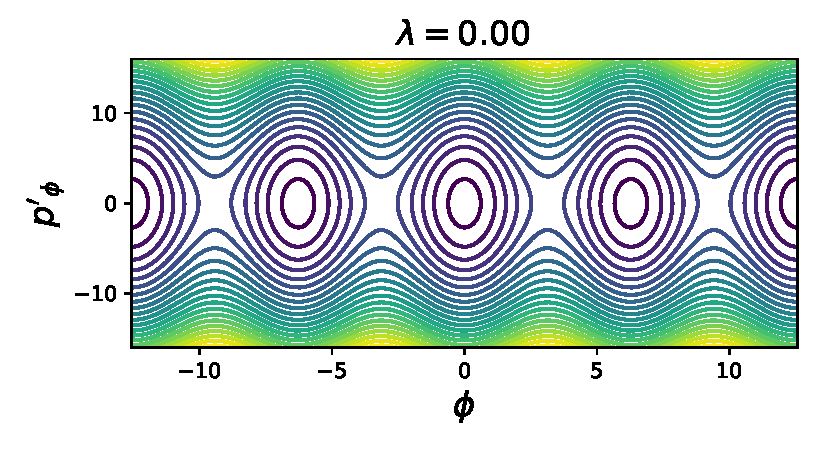
\includegraphics[width=0.49\textwidth]{{fig/lambd=0.00}.pdf}
    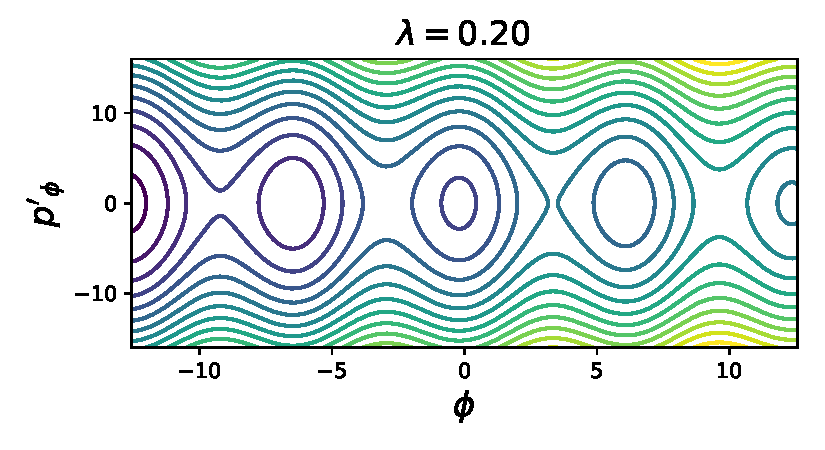
\includegraphics[width=0.49\textwidth]{{fig/lambd=0.20}.pdf}
    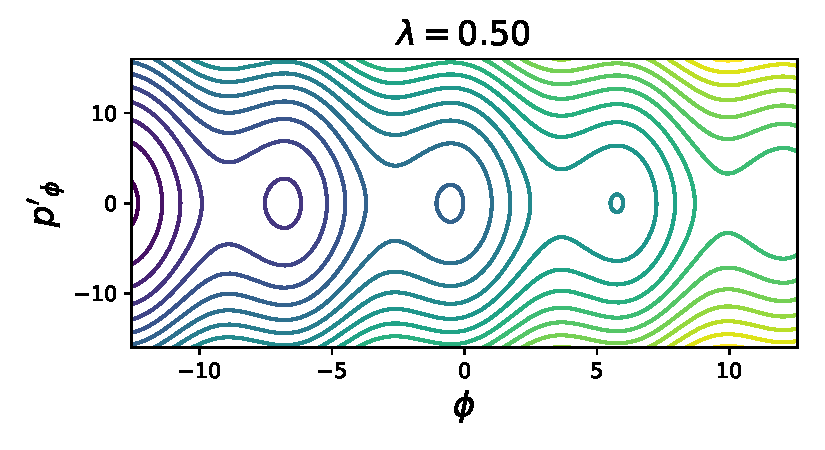
\includegraphics[width=0.49\textwidth]{{fig/lambd=0.50}.pdf}
    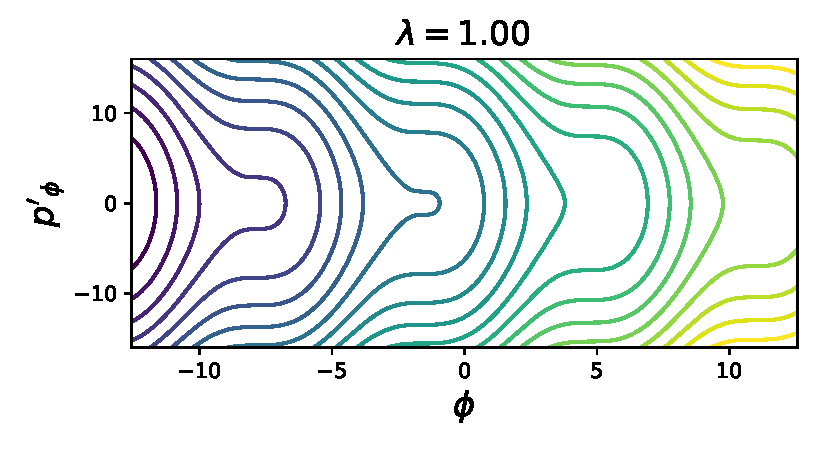
\includegraphics[width=0.49\textwidth]{{fig/lambd=1.00}.pdf}
    \caption{Contour plots of $H'(\phi, p'_\phi)$}
    \label{fig:contour}
\end{figure}

\begin{figure}[H]
    \centering
    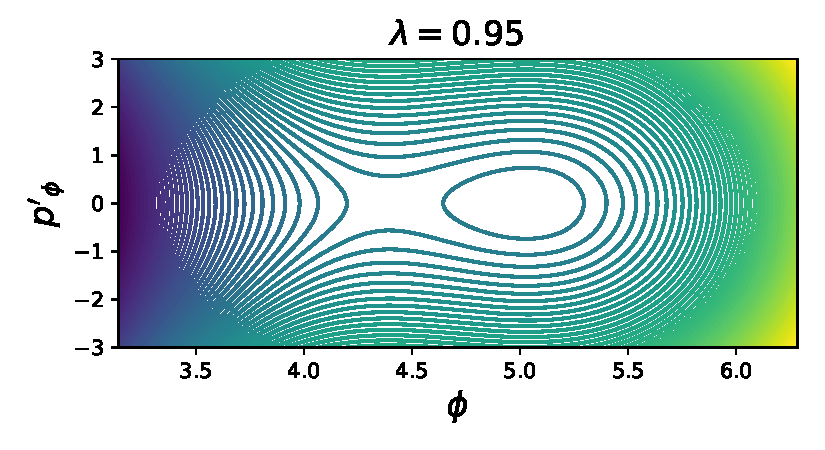
\includegraphics[width=0.49\textwidth]{{fig/x_lambd=0.95}.pdf}
    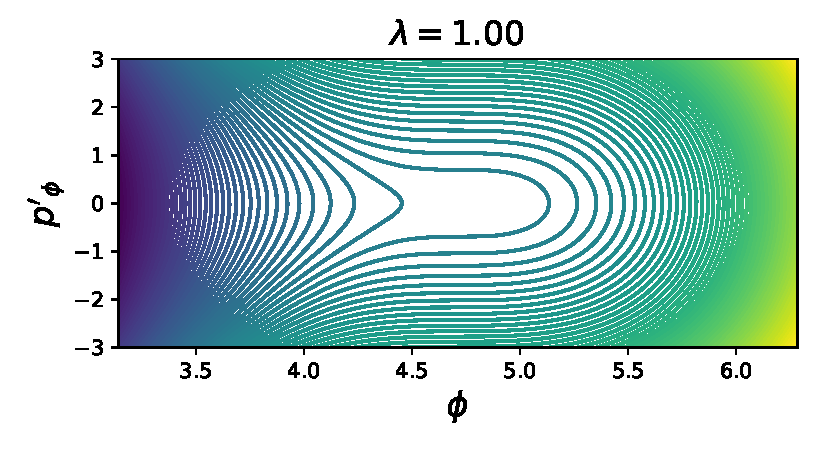
\includegraphics[width=0.49\textwidth]{{fig/x_lambd=1.00}.pdf}
    \caption{Higher density contour plots of $H'(\phi, p'_\phi)$}
    \label{fig:contour2}
\end{figure}



\section*{Oppgave 2}
\subsection*{a)}
The invariant mass $m_{ab}^2$ does not change between refrence frames because it is a Lorentz invariant quantity.

The sum of two momentum-energy four-vectors are also a four vector\footnote{see, for instance, \url{http://hyperphysics.phy-astr.gsu.edu/hbase/Relativ/vec4.html}}, meaning that $p_a + p_b$ is a four-vector. We also know that the length of a four-vector (defined as $x^2 = x^\mu x_\mu$) is a Lorentz invariant quantity. The quantity
\[
    m_{ab}^2c^2 = (p_a + p_b)^2 = (p_a + p_b)^\mu (p_a + o_b)_\mu
\]
must therefore be invariant. The invariant mass $m_{ab}^2$ is also invariant, as dividing by a constant $c^2$ does not break Lortentz invariace.

\subsection*{b)}
Conservation of energy gives that particle A and a must have a combined energy equal to that of particle B before the decacy.
\begin{align*}
    E_B &= E_A + E_a\\
    \sqrt{p_B^2c^2 + m_B^2c^4} &= \sqrt{p_A^2c^2 + m_A^2c^4} + \sqrt{p_a^2c^2 + m_a^2c^4}
\end{align*}
In the rest frame of A, $p_A = 0$, and conservation of momentum gives that $p_a^2 = p_B^2$ (total momentum before decay must equal total momentum after dacay). This gives

\begin{gather*}
    \sqrt{p_a^2 + m_B^2c^2} = \sqrt{m_A^2c^2} + \sqrt{p_a^2 + m_a^2c^2} \\
    \qty(\sqrt{p_a^2 + m_B^2c^2})^2 = \qty(\sqrt{m_A^2c^2} + \sqrt{p_a^2 + m_a^2c^2})^2 \\
    p_a^2 + m_B^2c^2 = m_A^2c^2 + p_a^2 + m_a^2c^2 + 2\sqrt{m_A^2c^2}\sqrt{p_a^2 + m_a^2c^2} \\
    \sqrt{p_a^2 + m_a^2c^2} = \frac{m_B^2c^2 - m_a^2c^2 - m_A^2c^2}{2m_Ac} \\
    p_a^2 + m_a^2c^2 = \frac{\qty(m_B^2c^2 - m_a^2c^2 - m_A^2c^2)^2}{4m_A^2c^2} \\
    p_a^2 + m_a^2c^2 = \frac{m_B^4c^4 + m_a^4c^4 + m_A^4c^4 - 2m_B^2m_a^2c^4 - 2m_B^2m_A^2c^4 + 2m_a^2m_A^2c^4}{4m_A^2c^2} \\
    p_a = \frac{\sqrt{m_B^4c^4 + m_a^4c^4 + m_A^4c^4 - 2m_B^2m_a^2c^4 - 2m_B^2m_A^2c^4 + 2m_a^2m_A^2c^4 - 4m_a^2m_A^2c^4}}{2m_Ac}
\end{gather*}
\begin{gather}\label{eqn:p_a}
    p_a = c\frac{\sqrt{m_B^4 + m_a^4 + m_A^4 - 2m_B^2m_a^2 - 2m_B^2m_A^2 - 2m_a^2m_A^2}}{2m_A}
\end{gather}


\subsection*{c)}
We have the invariant mass given as
\begin{gather*}
    m_{ab}^2c^2 = (p_a + p_b)^2 = (p_a + p_b)^\mu (p_a + p_b)_\mu
\end{gather*}

We write out the 4-vector with energy and regular momentum components
\begin{align*}
    (p_a + p_b)^\mu &= \qty(\frac{E_a + E_b}{c},\ \qty[\vec{p_a} + \vec{p_b}])\\
    (p_a + p_b)_\mu &= \qty(\frac{E_a + E_b}{c},\ -\qty[\vec{p_a} + \vec{p_b}])
\end{align*}
which gives the invariant mass
\begin{align*}
    m_{ab}^2c^2 = \frac{(E_a + E_b)^2}{c^2} - \qty[\vec{p_a} + \vec{p_b}]^2
\end{align*}
Inserting the relativistic energy (with $m_a = m_b = 0$)
\begin{align*}
    E_a &= \sqrt{p_a^2c^2 + m_a^2c^4} = p_ac \\
    E_b &= \sqrt{p_b^2c^2 + m_b^2c^4} = p_bc
\end{align*}
gives
\begin{align*}
    m_{ab}^2c^2 &= \frac{(p_ac + p_bc)^2}{c^2} - \qty[\vec{p_a} + \vec{p_b}]^2 \\
    &= p_a^2 + p_b^2 + 2p_ap_b - \vec{p_a}^2 - \vec{p_b}^2 - 2\vec{p_a}\cdot\vec{p_b}
\end{align*}
The squared vectors simply become their magnitudes squared ($\vec{p}^2 = p^2$), while the dot product can be written $\vec{p_a}\cdot\vec{p_b} = p_ap_b\cos{\theta_{ab}}$, where $\theta_{ab}$ is the angle between the vectors. This gives
\begin{align*}
    m_{ab}^2c^2 = 2p_ap_b - 2p_ap_b\cos{\theta_{ab}} = 2p_ap_b(1-\cos{\theta_{ab}})
\end{align*}
\begin{align}\label{eqn:m_ab}
    m_{ab}^2 = \frac{2}{c^2}p_ap_b(1-\cos{\theta_{ab}})
\end{align}

We observe that the decay $C \rightarrow bB$ from the refrence frame of $B$ is identical to the decay $B \rightarrow aA$ from the frence frame of $A$, solved in the last exercise. We therefore borrow equation (\ref{eqn:p_a}), substituting $(B, a, A)$ with $(C, b, B)$. Setting $m_b = 0$ gives
\begin{align}
    p_b = c\frac{\sqrt{m_C^4 + m_B^4 - 2m_C^2m_B^2}}{2m_B} = c\frac{\sqrt{(m_C^2 - m_B^2)^2}}{2m_B} = c\frac{m_C^2 - m_B^2}{2m_B}
\end{align}

We now need an expression for $p_a$.

Looking at the second decay from the refrence frame of $B$, we get the slightly different energy conservation, with $p_A^2 = p_a^2$ and $p_B = 0$. We also set $m_a = 0$.
\begin{gather*}
    E_B = E_A + E_a \\
    \sqrt{p_B^2c^2 + m_B^2c^4} = \sqrt{p_A^2c^2 + m_A^2c^4} + \sqrt{p_a^2c^2 + m_a^2c^4} \\
    \sqrt{p_B^2 + m_B^2c^2} = \sqrt{p_A^2 + m_A^2c^2} + \sqrt{p_a^2 + m_a^2c^2} \\
    m_Bc = \sqrt{p_a^2 + m_A^2c^2} + p_a \\
    (m_Bc - p_a)^2 = p_a^2 + m_A^2c^2 \\
    m_B^2c^2+ p_a^2 - 2m_Bp_ac = p_a^2 + m_A^2c^2
\end{gather*}
\begin{gather}
    p_a = c\frac{m_B^2 - m_A^2}{2m_B}
\end{gather}

Inserting this into equation (\ref{eqn:m_ab}) gives
\begin{align*}
    m_{ab}^2 = \frac{2}{c^2}c\frac{m_B^2 - m_A^2}{2m_B}c\frac{m_C^2 - m_B^2}{2m_B}(1-\cos{\theta_{ab}}) = \frac{(m_B^2 - m_A^2)(m_C^2 - m_B^2)}{2m_B^2}(1-\cos{\theta_{ab}})
\end{align*}



\subsection*{d)}
The idea is to use the following definitions of the invariant mass:
\begin{align*}
    m_{ab}^2 &= \frac{(p_a + p_b)^2}{c^2}\\
    m_{ac}^2 &= \frac{(p_a + p_c)^2}{c^2}\\
    m_{bc}^2 &= \dots
\end{align*}
To achive this, we need the maginutes of the four-momenta in the same refrence frame. We chose that of the particle E for this.

We start by solving for $p_a$ in reference frame of B (now with particles a and b having mass). This involves $p_B = 0$, and the momenta of a and A to be the same $p_A = p_a$.
\begin{gather*}
    E_B = E_A + E_a \\
    \sqrt{m_B^2c^4} = \sqrt{p_a^2c^2 + m_A^2c^4} + \sqrt{p_a^2c^2 + m_a^2c^4}
\end{gather*}
\begin{align}
    p_a = \frac{\sqrt{ c^4m_a^4 - 2c^4m_a^2m_B^2 + c^4m_B^4 - 2c^2m_A^2m_a^2 - 2c^2m_A^2 m_B^2 + m_A^4 }}{ 2cm_B }
\end{align}

Following the exact same logic, we find $p_b$ in reference frame of C.
\begin{align*}
    p_b &= \frac{\sqrt{ c^4m_b^4 - 2c^4m_b^2m_C^2 + c^4m_C^4 - 2c^2m_B^2m_b^2 - 2c^2m_B^2 m_C^2 + m_B^4 }}{ 2cm_C } \\
\end{align*}
The solutions of $p_c$ and $p_d$ in the refrence frames of D and E are similar, but two of the mass terms are zero: $m_c = m_d = 0$. The solutions becomes\footnote{$m_D > m_C$ and $m_E > m_C$, so we keep them in this order to get a positive absolute momentum.}
\begin{align*}
    p_c &= \frac{\sqrt{c^4m_D^4 - 2c^2m_C^2 m_D^2 + m_C^4 }}{ 2cm_D } = c\frac{m_D^2 - m_C^2}{2m_D} \\
    p_d &= \frac{\sqrt{c^4m_E^4 - 2c^2m_D^2 m_E^2 + m_D^4 }}{ 2cm_E } = c\frac{m_E^2 - m_C^2}{2m_E}
\end{align*}

The idea is now to Lorentz transform these four-momenta into the E refrence frame. To use a Lorentz transformation between the $A-B-C-D-E$ frames, we need their relative velocities.

We solve for $v_A$ in the refrence frame of B, using the definition $p = \gamma m v$ of the relativistic momentum, and employing that $p_a = p_A$ in the frame B.
\begin{gather*}
    p_a = p_A = \gamma_{AB}m_A v_A = \frac{1}{\sqrt{1-\frac{v_A^2}{c^2}}} m_A v_A \\
    p_a^2 = \frac{m_A^2 v_A^2}{1-\frac{v_A^2}{c^2}} \\
    p_a^2 - p_a^2\frac{v_A^2}{c^2} = m_A^2v_A^2 \\
    v_A^2(m_A^2 + \frac{p_a^2}{c^2}) = p_a^2 \\
\end{gather*}
\begin{equation}
    v_A = \frac{p_a}{\sqrt{m_A^2 + \frac{p_a^2}{c^2}}}
\end{equation}
The same logic can be applied to $v_B$ in the frame of C, and so forth:
\begin{equation}
    v_B = \frac{p_b}{\sqrt{m_B^2 + \frac{p_b^2}{c^2}}} \quad\quad
    v_C = \frac{p_c}{\sqrt{m_C^2 + \frac{p_c^2}{c^2}}} \quad\quad
    v_D = \frac{p_d}{\sqrt{m_D^2 + \frac{p_d^2}{c^2}}}
\end{equation}

We now introduce the general Lorentz matrix 
\begin{align*}
    L = 
    \begin{pmatrix}
        \gamma     &-\gamma\beta_x   &-\gamma\beta_y  &-\gamma\beta_z \\
        -\gamma\beta_x  &1+(\gamma-1)\frac{\beta^2_x}{\beta^2}  &(\gamma-1)\frac{\beta_x\beta_y}{\beta^2}   &(\gamma-1)\frac{\beta_x\beta_z}{\beta^2}\\
        -\gamma\beta_y  &(\gamma-1)\frac{\beta_y\beta_x}{\beta^2}  &1+(\gamma-1)\frac{\beta_y^2}{\beta^2}   &(\gamma-1)\frac{\beta_y\beta_z}{\beta^2}\\
        -\gamma\beta_z  &(\gamma-1)\frac{\beta_z\beta_x}{\beta^2}  &(\gamma-1)\frac{\beta_z\beta_y}{\beta^2}   &1+(\gamma-1)\frac{\beta_z^2}{\beta^2} 
    \end{pmatrix}
\end{align*}

to transform the four-momenta between refrence frames. Here we have the identities
\begin{align*}
    \beta_x = \frac{v_x}{c} \quad\quad \beta_y = \frac{v_y}{c} \quad\quad \beta_z = \frac{v_z}{c} \quad\quad \beta^2 = \frac{|v|^2}{c^2} \quad\quad \gamma = \frac{1}{\sqrt{1-\frac{v^2}{c^2}}}
\end{align*}

Since we only have information about the angles of the velocities, we use a transformation to achive the vector-velocities. We denote the angles between $a$ and $B$ as $\theta_a$ and $\phi_a$, and the angels between $A$ and $B$ as $\theta_A$ and $\theta_B$. Since the known (uniformily generated) angels are those of $a$, we transform these to $A$ as
\[
    \theta_A = \pi - \theta_a \quad\quad \phi_A = \pi + \phi_a
\]
This is due to $A$ and $a$ always having velocities in oposite directions in the frame of $B$ (due to momentum conservation). From here, we get the 3D vector components as

\begin{align*}
    \vec{v_A} = v_A\qty[\sin{\theta_A}\cos{\phi_A},\ \sin{\theta_A}\sin{\phi_A},\ \cos{\theta}]
\end{align*}
This can all easialy be translated to the other decays.

We wish the direction of decaying particles to uniformily distributed on a sphere. This does not, countrary to popular belief, correspond to a uniform distribution of the angles $\theta\in [0,\pi]$ and $\phi \in [0,2\pi]$. This is because an angular interval does not represent a fixed area on the sphere, and a uniform distribution would favor the poles. To create a uniform distribtion, we will employ the angles
\[
    \phi = 2\pi u   \quad\quad   \theta = \arccos(2v - 1)
\]
where $u$ and $v$ are uniform distributions in $[0, 1]$. This ensures an isotropic decay process.
\end{document}
